\section{Model, definitions and methods}\label{sec:model}

Evaluating protection by multiple hosts requires a specified life cycle, host-variability law, and baseline. We define these before introducing parasite feedback and the checking methods (Table~\ref{tab:model-notation}).

\subsection{The ring of stages}\label{sec:model-ring}

We model a rare parasite in discrete time ($t = 0, 1, 2, \dots$) across $n \ge 1$ sequential stages in a closed ring, reading stage indices modulo $n$ so that stage $n + 1$ is stage $1$ (Fig.~\ref{fig:intro-1}). With nonnegative continuous stage abundances $\mathbf{x}(t) = (x_1(t), \dots, x_n(t))^{\mathsf{T}}$, each individual in stage $k$ contributes a fixed staying amount $s_k \ge 0$ to stage $k$ and a transfer amount $g_k h_k(t)$ to stage $k + 1$. Here $g_k > 0$ is the baseline transfer and $h_k(t) > 0$ is a dimensionless host multiplier, giving
\begin{equation}\label{eq:model-ring}
x_{k+1}(t+1) = s_{k+1} x_{k+1}(t) + g_k h_k(t) x_k(t), \qquad \mathbf{x}(t+1) = \mathbf{A}(t)\mathbf{x}(t),
\end{equation}
where $\mathbf{A}(t)$ has diagonal entries $s_k$ and cyclic subdiagonal entries $g_k h_k(t)$ (or the single entry $s_1 + g_1 h_1(t)$ when $n = 1$). We adopt this gain-only formulation as our baseline because free-living or vector-borne stages often leave or perish at a constant rate regardless of host availability, so host scarcity wastes outgoing individuals rather than delaying exit (contact-limited waiting and multi-substage residence kernels $\widehat{K}(z)$ are analyzed in Section~\ref{sec:mech}). The factors $s_k$ and $g_k$ need not be probabilities, although expressions using ordinary lifetimes or $R_0$ require $0 \le s_k < 1$ for every $k$.

\begin{figure}[htbp]
\centering
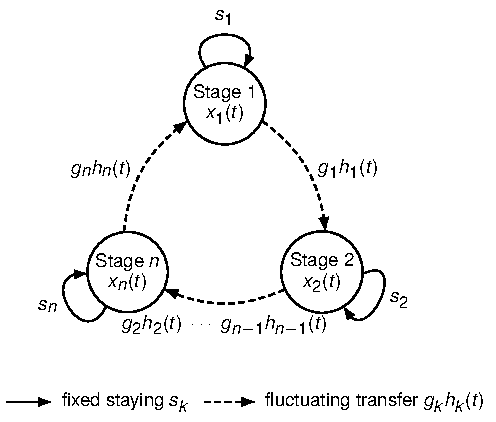
\includegraphics[width=84mm]{figures/intro-1.pdf}
\caption{Schematic of the discrete-time $n$-stage parasite life-cycle ring in~\eqref{eq:model-ring} (shown with stages $1$, $2$, and $n$ returning to stage $1$). Circular nodes represent sequential parasite stages with abundances $x_k(t)$, solid self-loops indicate fixed staying contributions $s_k \ge 0$, and dashed directed arcs indicate host-driven transfer contributions $g_k h_k(t)$ (fixing $h_k(t) \equiv 1$ gives a steady transfer)}\label{fig:intro-1}
\end{figure}

When $\E[h_k(t)] = 1$, the mean matrix $\mathbf{A}_0 = \E[\mathbf{A}(t)]$ is assumed primitive ($n = 1$, or $n \ge 2$ with at least one $s_k > 0$), with Perron root $\lambda = \spr(\mathbf{A}_0) > 0$ and positive right and left eigenvectors $\mathbf{v}$ and $\mathbf{w}$ normalized by $\mathbf{1}^{\mathsf{T}}\mathbf{v} = 1$ and $\mathbf{w}^{\mathsf{T}}\mathbf{v} = 1$. Where parallel host routes or staying and transfer terms share a matrix entry, we resolve them as finitely many labeled contributions $e$ from $j_e$ to $i_e$ with baseline weight $a_e > 0$ and fixed part $\mathbf{A}_{\mathrm{fixed}} \ge \mathbf{0}$,
\begin{equation}\label{eq:model-edges}
\mathbf{A}(t) = \mathbf{A}_{\mathrm{fixed}} + \sum_e a_e h_e(t)\mathbf{e}_{i_e}\mathbf{e}_{j_e}^{\mathsf{T}}, \qquad \mathbf{A}_0 = \mathbf{A}_{\mathrm{fixed}} + \sum_e a_e \mathbf{e}_{i_e}\mathbf{e}_{j_e}^{\mathsf{T}},
\end{equation}
where $\mathbf{e}_i$ is the $i$th unit vector. Following a line of descent forward weighted by reproductive value defines an irreducible, aperiodic reference Markov chain $P(j \to i) = w_i (\mathbf{A}_0)_{ij}/(\lambda w_j)$ with stationary law $\pi_k = w_k v_k$ \citep{bienvenu2015,bienvenu2017}. In~\eqref{eq:model-ring}, a reference lineage stays in stage $k$ with probability $m_k = s_k/\lambda$, giving geometric stays on $\{1, 2, \dots\}$ of mean $\tau_k = (1 - s_k/\lambda)^{-1} \ge 1$ (the lineage stay), circuit time $L$ of mean $\mathcal{T} = \sum_{k=1}^n \tau_k$ (the lineage generation time) and variance $\sum_{k=1}^n \tau_k(\tau_k - 1)$, and $\pi_k = \tau_k/\mathcal{T}$. At $\lambda = 1$ ($0 \le s_k < 1$), $\tau_k$ equals the ordinary mean stay $\tau_{k,0} = (1 - s_k)^{-1}$ and $\mathcal{T}$ equals $\mathcal{T}_0 = \sum_{k=1}^n \tau_{k,0}$. In continuous time, the gain-only ring is
\begin{equation}\label{eq:model-ct}
\frac{\mathrm{d}x_{k+1}}{\mathrm{d}t} = b_k \nu_k h_k(t) x_k(t) - (\nu_{k+1} + \mu_{k+1})x_{k+1}(t),
\end{equation}
with transfer exit rate $\nu_k > 0$, death rate $\mu_k \ge 0$, yield $b_k > 0$, mean-environment growth rate $r_0$, lineage exit rates $a_k = r_0 + \nu_k + \mu_k$, and generation time $T = \sum_{k=1}^n a_k^{-1}$.

\subsection{Host fluctuations}\label{sec:model-hosts}

In the baseline stochastic ring, hosts vary via stationary mean-one lognormal multipliers driven by first-order autoregressive (AR(1)) Gaussian processes,
\begin{equation}\label{eq:model-ar1}
h_k(t) = \exp\!\left(\sigma_k \xi_k(t) - \frac{\sigma_k^2}{2}\right), \qquad \xi_k(t+1) = \phi_k \xi_k(t) + \sqrt{1 - \phi_k^2}\,\epsilon_k(t+1),
\end{equation}
with independent innovations $\epsilon_k(t) \sim \mathcal{N}(0, 1)$, stationary $\xi_k(0) \sim \mathcal{N}(0, 1)$, log-abundance standard deviation (SD) $\sigma_k \ge 0$ (log variance $\sigma_k^2$, raw variance $\ee^{\sigma_k^2} - 1$), and lag-one log autocorrelation $\phi_k \in (-1, 1)$, giving $\E[h_k(t)] = 1$ and $\Cov(\xi_k(t), \xi_k(t-\ell)) = \phi_k^{|\ell|}$ (Fig.~\ref{fig:intro-2}). Positive geometric-memory comparisons take $0 \le \phi_k < 1$ with memory scale $\theta_k = \phi_k/(1 - \phi_k)$. Hosts are independent and unaffected by the parasite in the basic ring, whereas shared drivers $\delta(e)$ and real sensitivities $\kappa_e$ on edge $e$ use $h_e(t) = \exp(\sigma \kappa_e \xi_{\delta(e)}(t) - \sigma^2 \kappa_e^2/2)$ to preserve $\E[h_e(t)] = 1$.

\begin{figure}[htbp]
\centering
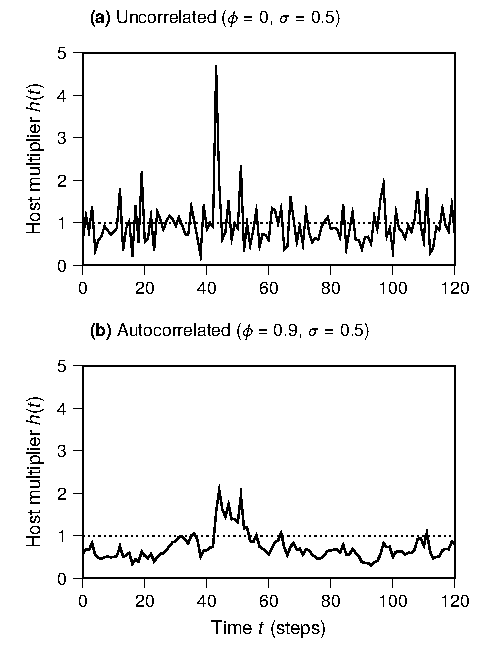
\includegraphics[width=84mm]{figures/intro-2.pdf}
\caption{Illustrative realizations of the mean-one lognormal host multiplier $h(t)$ in~\eqref{eq:model-ar1} over 120 steps with $\sigma = 0.5$ for (a) an uncorrelated host ($\phi = 0$) and (b) an autocorrelated host ($\phi = 0.9$). Solid curves use the same standard-Gaussian innovations and stationary start (seed 20261114), and horizontal dotted lines mark $\E[h(t)] = 1$ (synthetic model illustrations, not empirical host series)}\label{fig:intro-2}
\end{figure}

Four further environmental laws enter later sections. Sections~\ref{sec:ring} and~\ref{sec:mech} use jointly stationary centered unit-variance Gaussian linear processes $\xi_\delta(t) = \sum_{j=0}^{\infty} \psi_{\delta,j}\epsilon_\delta(t-j)$ with $\sum_{j=0}^{\infty} \psi_{\delta,j}^2 = 1$ and $\Psi_\delta = \sum_{j=0}^{\infty}|\psi_{\delta,j}| < \infty$ (covering damped second-order autoregressive (AR(2)) quasi-cycles and two-host Gaussian vector autoregressions). Continuous-time models in Section~\ref{sec:ring} use unit-variance Ornstein--Uhlenbeck (OU) log drivers $z_k(t)$ with covariance $\exp(-\alpha_k |t|)$ ($\alpha_k > 0$). Bounded-probability contact, thermal, and outage studies in Sections~\ref{sec:mech} and~\ref{sec:num} use two-state Markov multipliers $h(t) = 1 + \sigma\xi(t)$ ($\xi(t) \in \{-1, 1\}$), skewed two-state or on/off hosts, and periodic schedules of period $P$. Finally, Section~\ref{sec:exact} uses \citet{roerdink1988}'s two-stage ring $x_0(t+1) = g_1 x_1(t)$, $x_1(t+1) = s x_1(t) + g_0 h_t x_0(t)$ ($0 < s < 1$, $c = g_0 g_1 > 0$) with independent $h_t \sim \operatorname{Gamma}(p, 1/p)$ ($p > 0$, mean $1$, variance $1/p$).

\subsection{Reproduction number, baseline and loss}\label{sec:model-r0}

When $h_k(t) \equiv 1$, $g_k > 0$, and $0 \le s_k < 1$, designating $1 \le m \le n$ transfers as births splits $\mathbf{A}_0 = \mathbf{F} + \mathbf{V}$ ($\mathbf{F}$ holding the $m$ birth transfers and $\mathbf{V}$ the rest). The following proposition (proved below and refereed) links the whole-circuit number $R_0$, the next-generation number $R_{\mathrm{NG}}$, and $\lambda$.

\begin{proposition}[Birth convention and deterministic threshold]\label{prop:model-birth}
For the deterministic ring with $g_k > 0$, $0 \le s_k < 1$, and $1 \le m \le n$ designated birth transfers,
\begin{equation}\label{eq:model-r0}
R_0 = \prod_{k=1}^n \frac{g_k}{1 - s_k}, \qquad R_{\mathrm{NG}} = \spr\!\bigl(\mathbf{F}(\mathbf{I} - \mathbf{V})^{-1}\bigr) = R_0^{1/m}, \qquad \prod_{k=1}^n (\lambda - s_k) = \prod_{k=1}^n g_k,
\end{equation}
where $\mathbf{I}$ is the identity matrix. Counting every transfer gives $R_{\mathrm{NG}} = R_0^{1/n}$, the threshold is $R_0 = 1$ for every $m$, and $\ln\lambda = (\ln R_0)/\mathcal{T}_0 + O((\ln R_0)^2)$ as $\ln R_0 \to 0$ at fixed $s_k$ (exact at all $R_0$ when $n = 1$ and $s_1 = 0$).
\end{proposition}

\begin{proof}
Dividing the $m$ birth transfers by $R > 0$ gives $\prod_{k=1}^n (\lambda - s_k) = R^{-m}\prod_{k=1}^n g_k$. Setting $\lambda = 1$ yields $R^m = R_0$, so $R_{\mathrm{NG}} = R_0^{1/m}$ and $R_{\mathrm{NG}} = 1 \iff R_0 = 1$. Differentiating $\sum_{k=1}^n \ln[(\lambda - s_k)/(1 - s_k)] = \ln R_0$ with respect to $\ln\lambda$ at $\lambda = 1$ gives $\mathcal{T}_0 > 0$, yielding $\ln\lambda = (\ln R_0)/\mathcal{T}_0 + O((\ln R_0)^2)$ (exact when $n = 1, s_1 = 0$).
\end{proof}

Our default baseline fixes every rate at its arithmetic mean ($\E[h_e(t)] = 1$, giving $\mathbf{A}_0$). Alternative baselines fix lognormal hosts at their geometric mean (Section~\ref{sec:bounds}), host abundance at $\overline{H}$ inside an encounter curve $F(H)$ (Section~\ref{sec:mech}), or temperature at $\overline{T}$ inside thermal rates (Section~\ref{sec:mech}), and can reverse an effect's sign.

For a fixed nonzero nonnegative initial vector $\mathbf{x}(0)$ independent of future environments under stationary ergodic forcing with integrable logarithms, write $r = \lim_{t\to\infty} t^{-1}\ln\|\mathbf{x}(t)\|$. Adopting the zero-growth birth-divisor characterization of \citet{bacaer2013}, let $R_0^*$ be the common positive divisor on the $m$ birth transfers giving $r = 0$, and define
\begin{equation}\label{eq:model-loss}
\mathrm{cost} = \ln\lambda - r, \qquad D = \ln R_0 - m\ln R_0^*, \qquad \ln R_0^* = \frac{\ln R_0 - D}{m}.
\end{equation}
We write $C$ (or $C''$) for the $\sigma^2$ coefficient of $\mathrm{cost}$ and $\Gamma = \mathcal{T} C \sigma^2$ (summed over independent hosts) for the second-order term of the per-generation loss $\mathcal{T}(\ln\lambda - r)$. Non-ring networks use $\Delta$, the log restoring birth multiplier relative to threshold ($D = m\Delta$ in a ring). Negative losses are called gains, and neither $D$ nor $\Gamma$ is an integer-population extinction probability. The next proposition (proved below and refereed) establishes existence and invariance of $D$ in the lognormal AR(1) ring.

\begin{proposition}[Existence and invariance of the ring threshold loss]\label{prop:model-loss}
In~\eqref{eq:model-ring} with fixed $0 \le s_k < 1$ ($n = 1$, or $n \ge 2$ with some $s_k > 0$), $g_k > 0$, $1 \le m \le n$ birth transfers, and stationary AR(1) lognormal multipliers~\eqref{eq:model-ar1} with $|\phi_k| < 1$, $R_0^*$ exists uniquely and $D$ depends only on $(s_1, \dots, s_n)$ and the multiplier law, not on $(g_1, \dots, g_n)$ or $m$.
\end{proposition}

\begin{proof}
Rescaling $x_k \mapsto d_k x_k$ ($d_k > 0$) replaces $g_k$ by $g_k d_{k+1}/d_k$ without changing $s_k$, $h_k(t)$, or $r$, so $r$ depends only on $y = \ln\prod_{k=1}^n g_k$, written $r(y)$. Dividing $m$ births by $R$ shifts $y$ to $y - m\ln R$, so at a unique root $r(y_0) = 0$ we have $D = y_0 - \sum_{k=1}^n \ln(1 - s_k)$, independent of $g_k$ and $m$. If $n = 1$ and $s_1 = 0$, $r(y) = y - \sigma_1^2/2$ gives unique $y_0 = \sigma_1^2/2$. Otherwise some $s_k > 0$. Setting $g_k = c_k \ee^{y/n}$ ($\prod_{k=1}^n c_k = 1$), each path of length $t$ with $j$ transfers carries $\ee^{j y/n}$ times a positive weight, making $\ln\|\mathbf{x}(t)\|$ and hence $r(y)$ convex and nondecreasing. Integrable lognormal norms and the never-transferring path give $\max_k \ln s_k \le r(y) < \infty$, so $r(y)$ is finite and continuous. Since $r(y) \le \E[\ln\max_k(s_k + c_k \ee^{y/n} h_k(0))] \to \max_k \ln s_k < 0$ as $y \to -\infty$ and the always-transferring path gives $r(y) \ge y/n + c_0 \to +\infty$ as $y \to +\infty$ (finite $c_0$), a root exists, and convexity with a negative left limit rules out two roots.
\end{proof}

Along a fixed noise direction in this ring, Section~\ref{sec:ring} proves $D = \Gamma_0 + O(\sigma^4)$, where $\Gamma_0$ evaluates $\Gamma$ at $\tau_{k,0} = (1 - s_k)^{-1}$ ($\Gamma \ne \Gamma_0$ in general away from threshold).

\subsection{Hosts with their own dynamics}\label{sec:model-dyn}

When an established parasite affects host prevalence or survival (Section~\ref{sec:dyn}), we model a continuous-time ring of $n$ blocks coupled solely through scalar infection pressure ($u_k$ entering block $k$, $v_k = u_{k+1}$ leaving it). Around a positive equilibrium, local stability requires all linearized eigenvalues to have negative real part and is governed by each block's relative linear frequency response $E_k(z) = N_k(z)/D_k(z)$ (derived independently twice, checked numerically by a third party, and refereed). The first three blocks are an unregulated stage ($\mathrm{L}$, $\dot{w} = u - a w$, $v = c w$, $E_{\mathrm{L}} = a/(z + a)$), a regulated transfer ($\mathrm{R}$, $v = c f(w) w$, $\kappa = -w^* f'(w^*)/f(w^*)$, $E_{\mathrm{R}} = (1 - \kappa)a/(z + a)$), and a constant-size host ($\mathrm{S}$, $\dot{I} = u(N - I) - a I$, $v = c I$, prevalence $p = I^*/N \in (0, 1)$, $E_{\mathrm{S}} = a/[z + a/(1 - p)]$). The two dynamic-host blocks are a susceptible--infected host killed at rate $\alpha > 0$ ($\mathrm{V}$, $\dot{N} = \Phi(N) - \alpha I$, $\dot{I} = u(N - I) - a I$, $v = c I$, requiring $a \ge \alpha$, with $\rho = -\Phi'(N^*)$, $q = a$, $d = a/(1 - p)$, $h = \alpha p$) and a macroparasite host after \citet{anderson1978} ($\mathrm{M}$, $\dot{H} = \Phi(H) - \alpha P$, $\dot{P} = u H - \xi P - \alpha \varepsilon P^2/H$, $v = \lambda_P P$, $\varepsilon \ge 1$, mean burden $m = P^*/H^*$, $\rho = -\Phi'(H^*)$, $h = \alpha m$, $q = \xi + \varepsilon h$, $d = \xi + 2\varepsilon h$). Blocks $\mathrm{V}$ and $\mathrm{M}$ and the cycle characteristic polynomial satisfy
\begin{equation}\label{eq:model-blocks}
E_{\mathrm{V,M}}(z) = \frac{q(z + \rho)}{(z + \rho)(z + d) + d h}, \qquad \chi(z) = \prod_{k=1}^n D_k(z) - \prod_{k=1}^n N_k(z),
\end{equation}
retaining internal modes that can cancel in $\prod_{k=1}^n E_k(z) = 1$.

\begin{table}[t]
\caption{Summary of principal notation, meanings, and units}\label{tab:model-notation}
{\scriptsize\setlength{\tabcolsep}{0.5pt}
\begin{tabular*}{\textwidth}{@{\extracolsep{\fill}}llll@{}}
\toprule
Symbol & Meaning & Units & First use \\
\midrule
$x_k, \mathbf{x};\, X_k$ & Stage amount, vector; local population variable & Population & \eqref{eq:model-ring}, \S\ref{sec:dyn} \\
$n, k$ & Number of stages in ring; stage index (mod $n$) & Dimless & \eqref{eq:model-ring} \\
$s_k, g_k$ & Staying and transfer multipliers per census step & Dimless & \eqref{eq:model-ring} \\
$h_k(t), \xi_k(t)$ & Mean-one host multiplier; standardized log driver & Dimless & \eqref{eq:model-ring}, \eqref{eq:model-ar1} \\
$\sigma_k, \phi_k$ & Log-host SD and lag-1 correlation & Dimless & \eqref{eq:model-ar1} \\
$\theta_k$ & Memory scale $\phi_k/(1-\phi_k)$ & Steps & \S\ref{sec:model-hosts} \\
$\kappa_e$ & Signed noise sensitivity on labeled edge $e$ & Dimless & \S\ref{sec:model-hosts} \\
$p$ & Gamma shape in \S\ref{sec:exact}; prevalence in \S\ref{sec:dyn} & Dimless & \S\ref{sec:model-hosts}, \S\ref{sec:model-dyn} \\
$\nu_k, \mu_k, \alpha_k$ & Continuous transfer exit, death, and OU rates & Time$^{-1}$ & \eqref{eq:model-ct}, \S\ref{sec:model-hosts} \\
$b_k$ & Baseline descendants per transfer or leaver & Event$^{-1}$ & \eqref{eq:model-ct}, \S\ref{sec:num} \\
$u, v, E(z)$ & Block infection input, output, frequency response & Block, dimless & \S\ref{sec:model-dyn} \\
$\rho = -\Phi'$ & Negative slope of host total net production & Time$^{-1}$ & \S\ref{sec:model-dyn} \\
$\alpha, \varepsilon$ & Infection host death rate; burden clumping & Time$^{-1}$, dimless & \S\ref{sec:model-dyn} \\
$c, \mu$ & Contact and waiting-death probabilities per step & Dimless & \S\ref{sec:mech} \\
$T_t, \sigma_T$ & Daily temperature and temperature SD & $^{\circ}\mathrm{C}$ & \S\ref{sec:mech} \\
$\widehat{K}(z), K(\ell)$ & Sheltered kernel transform and lag-$\ell$ mass & Descendants & \S\ref{sec:model-ring}, \S\ref{sec:mech} \\
$\mathbf{A}_0, \lambda, \mathbf{v}, \mathbf{w}$ & Mean matrix, Perron root, right/left eigenvectors & Map, vectors & \eqref{eq:model-edges} \\
$r, r_0$ & Stochastic and mean-environment log growth rates & Rate & \eqref{eq:model-ct}, \eqref{eq:model-loss} \\
$\tau_k, \mathcal{T}, \mathcal{T}_0$ & Lineage stay, lineage and threshold gen.\ times & Steps & \S\ref{sec:model-ring} \\
$R_0, R_{\mathrm{NG}}, R_0^*$ & Circuit $R_0$, $m$-birth $R_0$, stochastic divisor & Dimless & \eqref{eq:model-r0}, \eqref{eq:model-loss} \\
$\mathrm{cost}, \Gamma, D, \Delta$ & Step loss, $\sigma^2$ gen.\ loss, $\ln R_0$ loss, shift & Log units & \eqref{eq:model-loss} \\
$J, J_2$ & Thermal curvature shift or lineage log-penalty rate & Log units & \S\ref{sec:model-methods}, \S\ref{sec:mech} \\
$\mathbf{B}_e, c_e, \mathbf{Q}, \mathbf{T}_\perp$ & Edge matrix, edge frequency, projection, transverse & Dimless & \eqref{eq:model-c2} \\
$C, C''$ & Second-order per-step growth-cost coefficients & Step$^{-1}\sigma^{-2}$ & \eqref{eq:model-c2} \\
$\rho_{\delta\delta'}(\ell)$ & Directed lag-$\ell$ covariance $\E[\xi_\delta(t)\xi_{\delta'}(t-\ell)]$ & Dimless & \eqref{eq:model-c2} \\
$V_2$ & Unscaled within-environment lineage variance rate & Step$^{-1}$ & \S\ref{sec:model-methods}, \S\ref{sec:bounds} \\
$P$ & Environmental period (distinct from burden $P$) & Steps & \S\ref{sec:model-hosts} \\
\bottomrule
\end{tabular*}}
\end{table}

\subsection{Methods of derivation and checking}\label{sec:model-methods}

On~\eqref{eq:model-edges} with primitive $\mathbf{A}_0$ and $h_e(t) = \exp(\sigma \kappa_e \xi_{\delta(e)}(t) - \sigma^2 \kappa_e^2/2)$, set $\mathbf{M} = \mathbf{A}_0/\lambda$, $\mathbf{Q} = \mathbf{I} - \mathbf{v}\mathbf{w}^{\mathsf{T}}$, $\mathbf{T}_\perp = \mathbf{M} - \mathbf{v}\mathbf{w}^{\mathsf{T}}$, $\mathbf{B}_e = (a_e/\lambda)\mathbf{e}_{i_e}\mathbf{e}_{j_e}^{\mathsf{T}}$, $c_e = \mathbf{w}^{\mathsf{T}}\mathbf{B}_e\mathbf{v}$, and $\rho_{\delta\delta'}(\ell) = \E[\xi_\delta(t)\xi_{\delta'}(t-\ell)]$. The published second-order coefficient \citep{ruelle1979,tuljapurkar1982a,tuljapurkar2006} and discrete-time lognormal remainder bound (proved and refereed for Gaussian linear processes with $\Psi_\delta < \infty$ in Section~\ref{sec:ring} and Appendix~A, with uniform AR(1) constants on compact families via Lemma~U and separate $O(|\sigma|^3)$ or symmetric $O(\sigma^4)$ bounded-driver remainders) are
\begin{align}
C'' &= \sum_{e,e'} \kappa_e \kappa_{e'}\biggl[\frac{c_e c_{e'}}{2}\rho_{\delta(e)\delta(e')}(0) \nonumber\\
&\qquad\qquad - \sum_{j=0}^{\infty} \rho_{\delta(e)\delta(e')}(j+1)\,\mathbf{w}^{\mathsf{T}}\mathbf{B}_e \mathbf{T}_\perp^j \mathbf{Q}\mathbf{B}_{e'}\mathbf{v}\biggr], \label{eq:model-c2}\\
\bigl|\ln\lambda - r(\sigma) - C''\sigma^2\bigr| &\le K\sigma^4 \qquad (|\sigma| \le \sigma_0). \label{eq:model-rem}
\end{align}
Constants $K$ and $\sigma_0$ are non-explicit, and continuous-time or thermal expansions give formal coefficients only. Strict coefficient inequalities transfer to small $|\sigma|$ where~\eqref{eq:model-rem} holds, whereas equal coefficients do not settle finite-noise order. Section~\ref{sec:bounds} uses path expansions on $P$ with reward $S_T = \sum_{t=1}^T \ln h_{e_t}(t)$ to prove $r - \ln\lambda \ge -\sum_e c_e \ell_e$ ($\ell_e = -\E[\ln h_e]$) and rewrite $C''\sigma^2 = \sigma^2(J_2 - \tfrac{1}{2}V_2)$ via $J_2 = \tfrac{1}{2}\sum_e c_e \kappa_e^2$ and within-environment lineage reward variance rate $\sigma^2 V_2$. Exact checks use periodic monodromy products $\boldsymbol{\mathcal{F}} = \mathbf{A}(P-1)\cdots\mathbf{A}(0)$ ($r_P = P^{-1}\ln\spr(\boldsymbol{\mathcal{F}})$; \citealp{bacaer2007}) and \citet{roerdink1988}'s Kummer density and Tricomi $U(p, b, \kappa)$ growth formula (Section~\ref{sec:exact}).

Simulations followed written protocols with tolerances fixed beforehand. Core ring and coupled-host equations had independent derivations, second-party code reproductions, and referee checks. The Cary Institute and National Ecological Observatory Network (NEON) analyses were computed once. Lean~4 checked the statements and components listed in the reconciled coverage inventory archived with the Lean sources (see Code availability). Some model identifications, stochastic limits and remainder estimates remain outside that coverage and rely on written proofs. Numerical settings and validation logs are given in Online Resource~1.

\subsection{Use of large language models}\label{sec:model-llm}

{\sloppy
All derivations, proofs, simulation and verification scripts, literature searches and reading cards, referee reports, Lean~4 formalizations, and manuscript text were produced by large language model systems (Claude, Anthropic; Codex, OpenAI; and a Gemini-based agent run through Cursor, here called Carbon). Separate model instances derived core results without access to each other's intermediate work. Second-party scripts reproduced closed forms and simulations from specifications, followed by referee audits and Lean checks (Section~\ref{sec:model-methods}; details in Online Resource~1). These checks do not replace human accountability or specialist review. No person is recorded as having checked a derivation, simulation, literature card, or formal proof file. The author reviewed the worked example and the verification records and approved the manuscript.\par}
